\section{Ground Truth for Clustering} \label{sec:Comparison_Clustering}

To further investigate in the source of the errors \autoref{fig:PCA_Cluster_Knee_4} \textbf{\textsf{B}} and \textbf{\textsf{D}}, \gls{HDBSCAN} was performed in a more simple manner, without $\varepsilon$ exploration on the small subset of H13 and H16 cluster of segment 4 in \autoref{fig:PCA_Clusteree_Knee_4}. Three different input matrices were used to compare the clustering by \gls{HDBSCAN} and find a ground truth. The first input was the non-reduced set of k-mer frequency vectors used in \autoref{sec:K_mer_Representation} as precalculated matrix with cosine distance (\autoref{sec:MAFFT}). Clustering was then performed and the result visualized as a cluster-tree (\autoref{fig:Simple_Clustertree_Cosine}). 

\begin{figure}[!hbt]
    \centering
    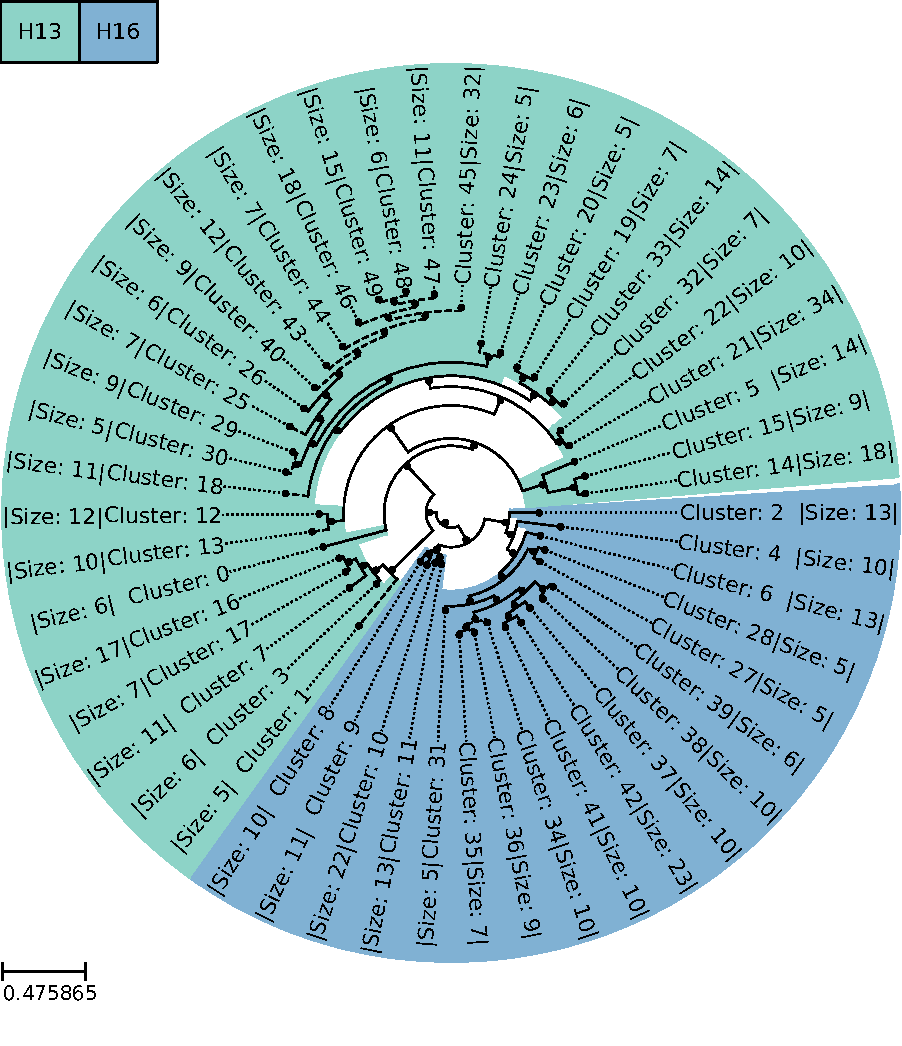
\includegraphics[width=\textwidth]{PCA/Clustertree_Segment_4_H_Cosine.pdf}
    \caption[H13/H16 simple precalculated cosine distance cluster tree]{\textbf{H13/H16 simple cosine distance cluster tree.} Cluster tree, based on the clustering by simple \gls{HDBSCAN} without any $\varepsilon$ exploration and hybrid clustering. The matrix used contained precalculated cosine distances of all the k-mer frequency vectors to each other. The used vectors were calculated from the sequences, present in the H13 and H16 clusters in \autoref{fig:PCA_Clusteree_Knee_4} without reduction with \gls{PCA} or \gls{UMAP}. Therefore, \gls{HDBSCAN} was used with precalculation input instead of a distance metric.}
    \label{fig:Simple_Clustertree_Cosine}
\end{figure}

\begin{figure}[!hbt]
    \centering
    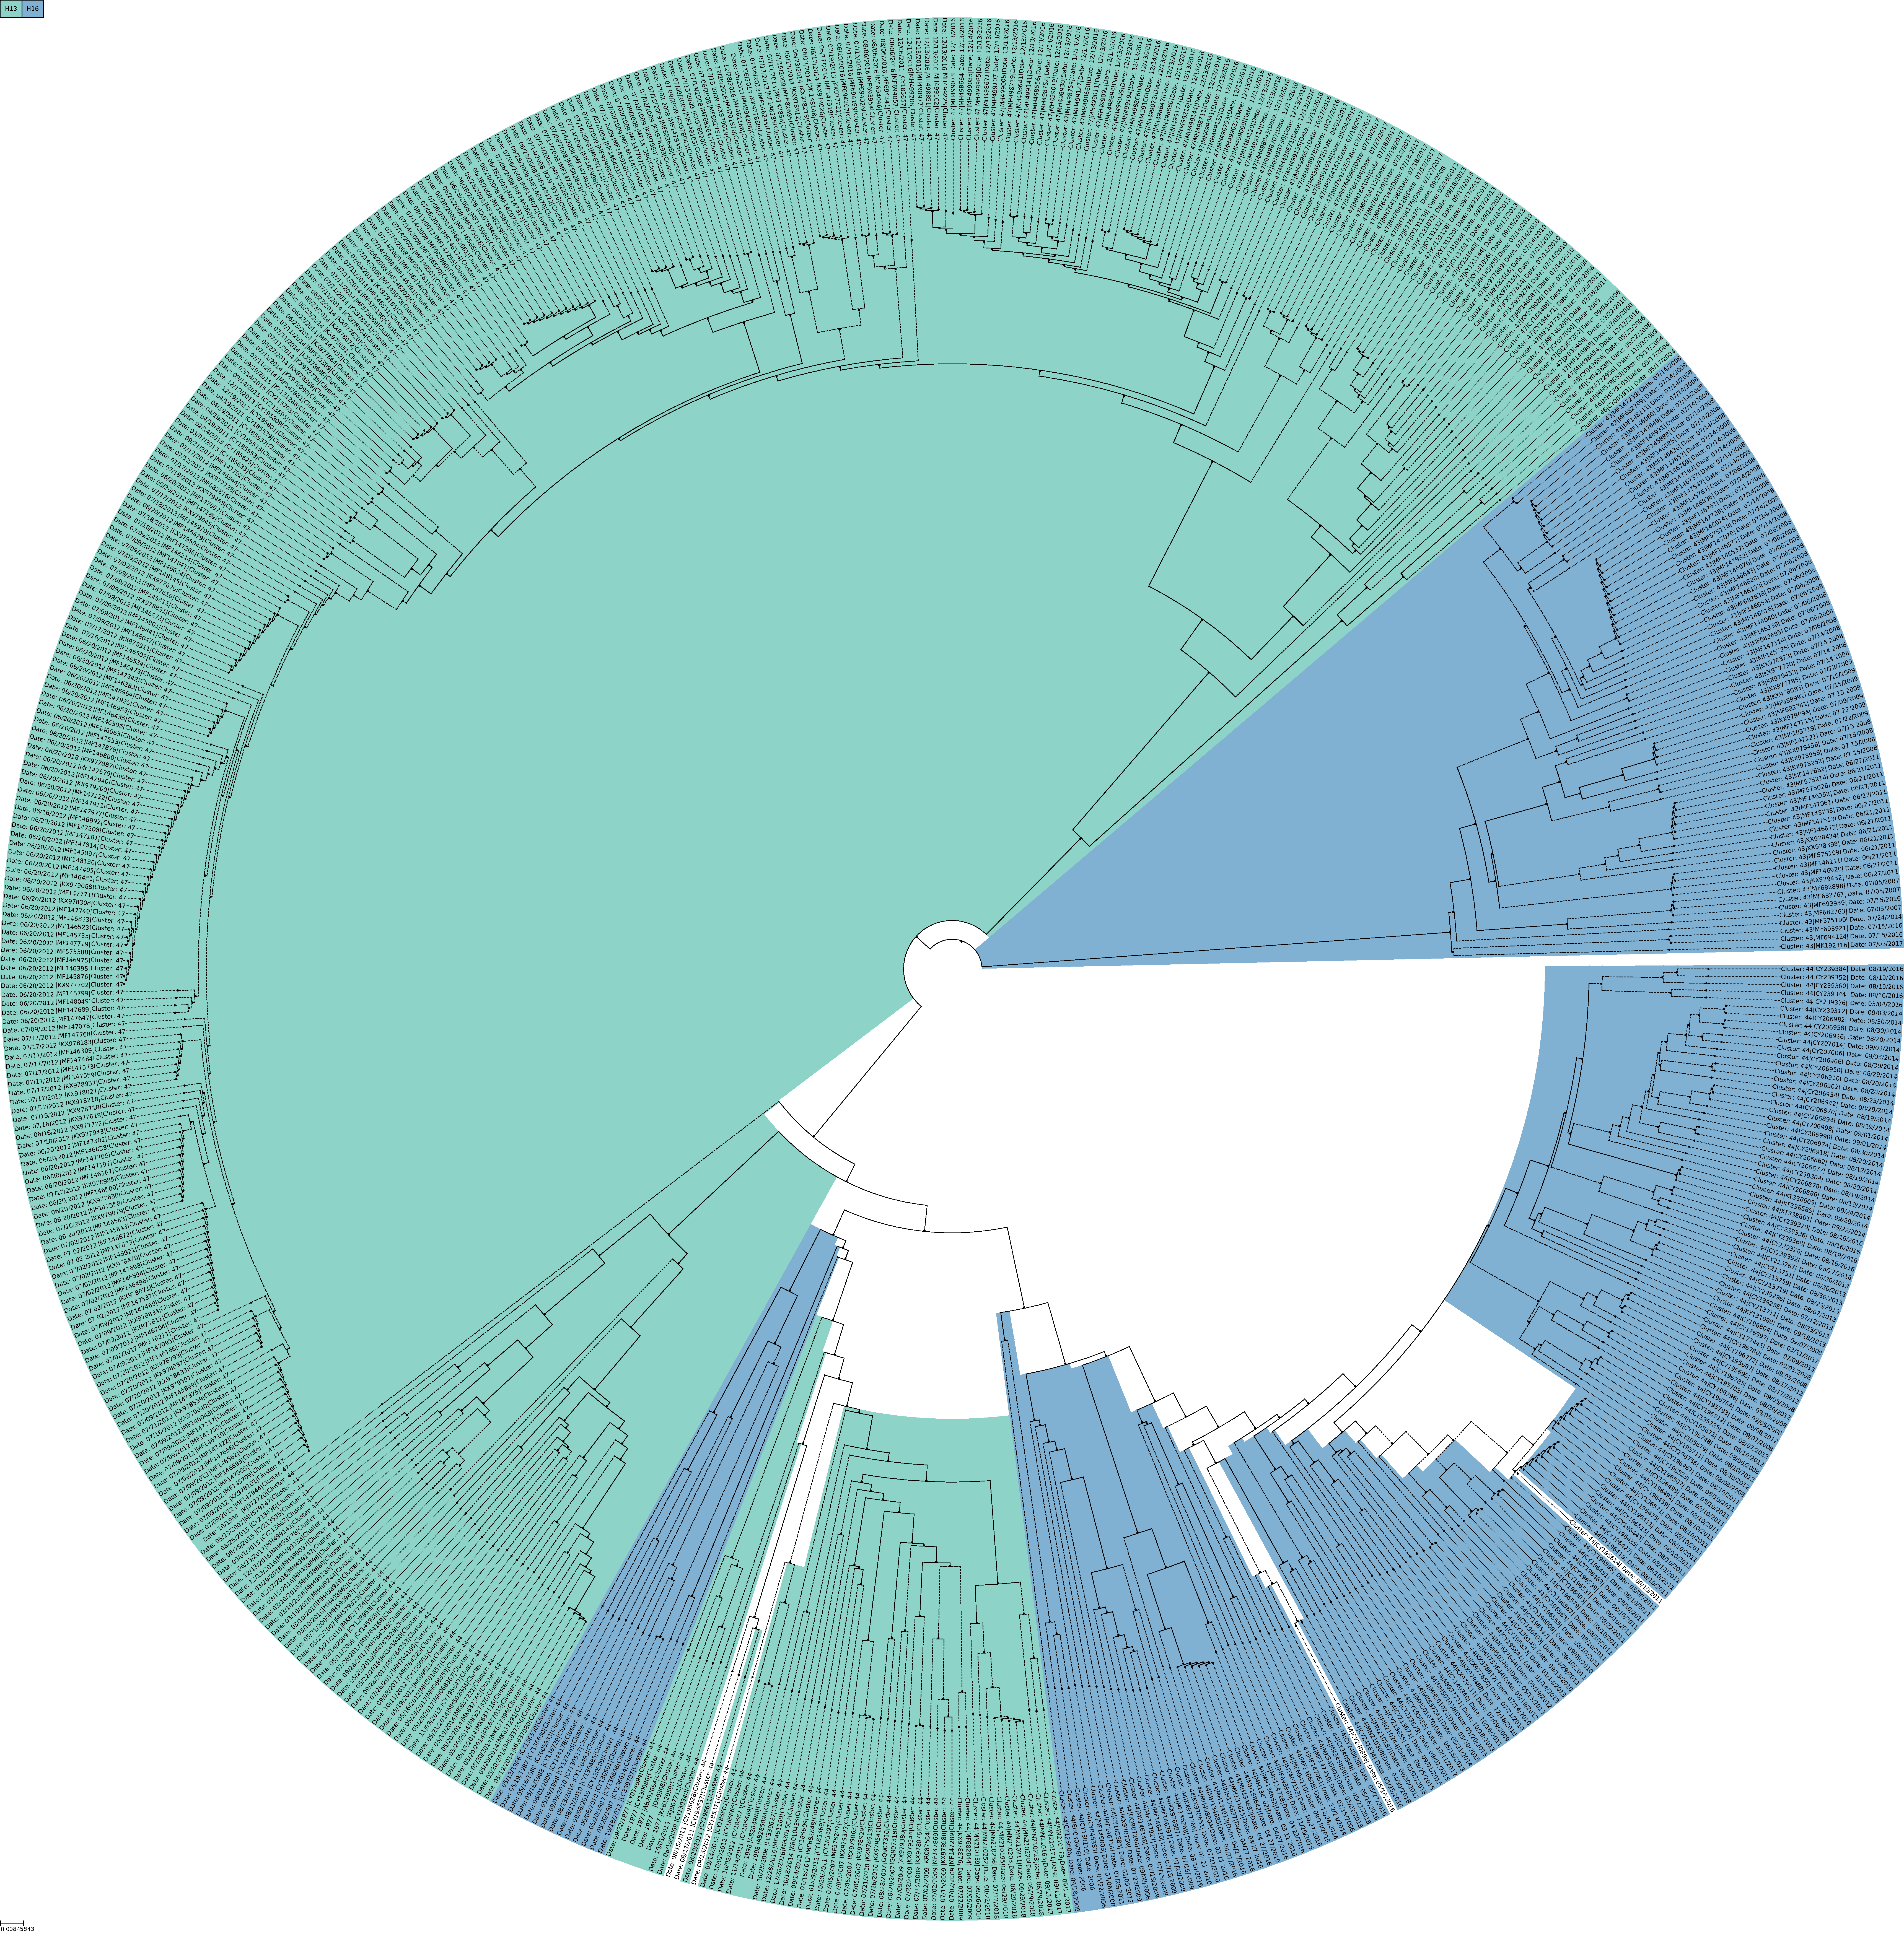
\includegraphics[width=\textwidth]{PCA/Clustertree_Segment_4_H_Focus.pdf}
    \caption[H13/H16 simple precalculated \gls{MSA} distance cluster tree]{\textbf{H13/H16 simple precalculated \gls{MSA} distance cluster tree.} Cluster tree, based on the clustering by simple \gls{HDBSCAN} without any $\varepsilon$ exploration and hybrid clustering. The matrix used contained precalculated \gls{MSA} based distances of all the sequences to each other. The sequences, present in the H13 and H16 clusters in \autoref{fig:PCA_Clusteree_Knee_4} were used for the \gls{MSA}. Therefore, \gls{HDBSCAN} was used with precalculation input instead of a distance metric.}
    \label{fig:Simple_Clustertree_MSA}
\end{figure}

\begin{figure}[!hbt]
    \centering
    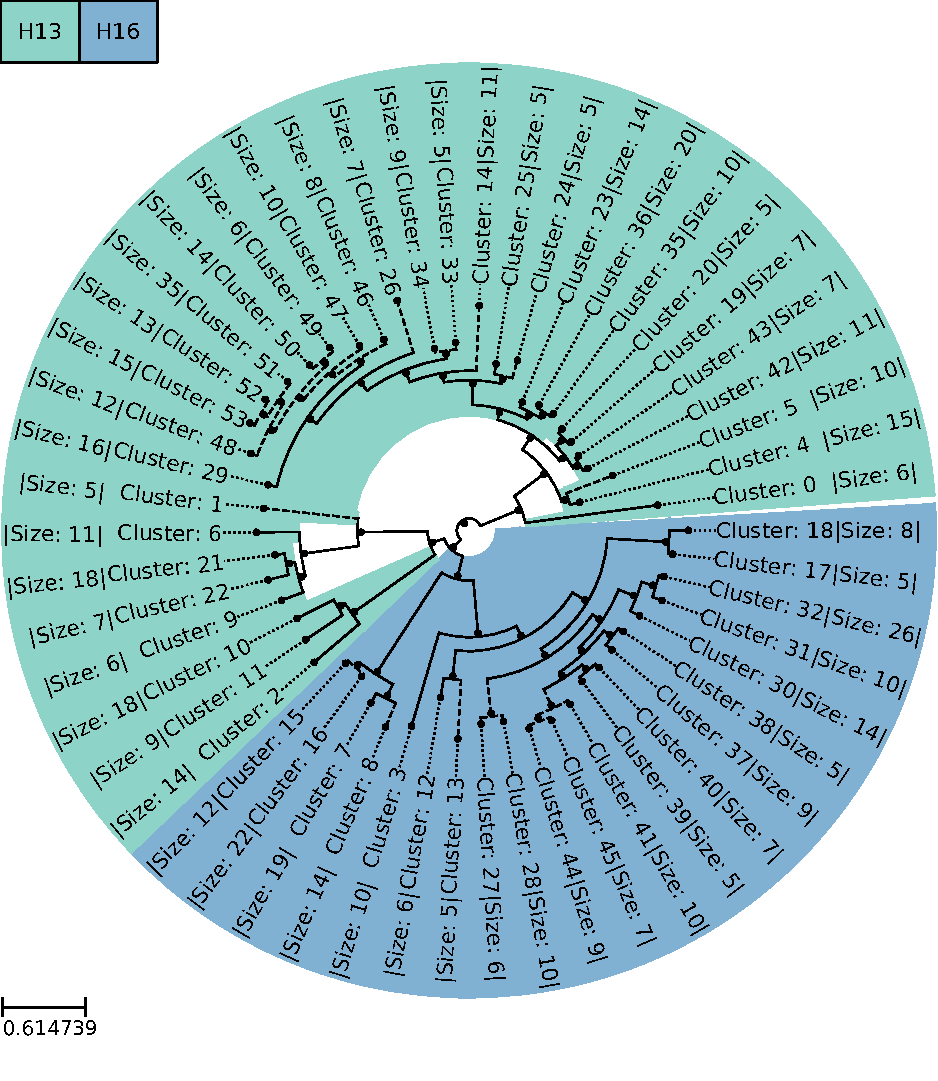
\includegraphics[width=\textwidth]{PCA/Clustertree_Segment_4_H_Simple.pdf}
    \caption[H13/H16 Simple \Acrshort{PCA} vector distance cluster tree]{\textbf{H13/H16 Simple \Acrshort{PCA} vector distance cluster tree.} Cluster tree, based on the clustering by simple \gls{HDBSCAN} without any $\varepsilon$ exploration and hybrid clustering. The used vectors were calculated from the sequences, present in the H13 and H16 clusters in \autoref{fig:PCA_Clusteree_Knee_4} with prior \gls{PCA} reduction to 30 dimensions.}
    \label{fig:Simple_Clustertree_PCA}
\end{figure}

In a similar manner to the precalculated \gls{UPGMA} tree in \autoref{fig:Precalculated_Cosine}, the subtypes are completely separated and split on both sides in two subgroups. This points to the fact, that the \gls{HDBSCAN} clustering of the precalculated cosine distances of the k-mer frequencies are as usable as the k-mer frequencies itself and are able to draw a clear line to separate the subtypes. This finding is in line with the second simple cluster-tree based on the evolutionary distances of a \gls{MSA} containing the same sequences as used in the former precalculated cosine distance clustering (\autoref{fig:Simple_Clustertree_MSA}). The same separation is even more obvious, as the subtypes are farther away from the separation at the trees root. On the side of the H13 sequences, a subdivision is also as clear as the subtype separation. Subgroups in the H16 sequences are, on the other hand, not that clear in \autoref{fig:Simple_Clustertree_MSA}. Maybe the different distances between the subtypes and the subgroups on each side of the subtypes is different because evolutionary aspects like weightings and different costs for nucleotides that are more likely to change are used. In the k-mer frequencies, the pure constellation of nucleotides is used, evolutionary aspects are neglected. Both, the precalculated approach as well as the \gls{MSA} evolutionary distances used the full information available from the sequences themselves, since no reduction with \gls{PCA} was performed. Therefore these cluster trees (\autoref{fig:Simple_Clustertree_Cosine} and \autoref{fig:Simple_Clustertree_MSA}) are the only ground truth for H13/H16 clustering with \gls{HDBSCAN} available. Precalculated clustering with \gls{HDBSCAN} as performed, is a highly computationally expensive task, as with $n$ sequences, the matrices of size $n^2$ have to be calculated and saved to be used in \gls{HDBSCAN}. The calculation is, therefore, not possible without the availability of major RAM space. When using \gls{HDBSCAN} with the k-mer vectors posterior to reduction with \gls{PCA} to 30 dimensions, only a matrix of size $n\times 30$ has to be saved without the necessity of any distance precalculation. To find a clustering method available without using hardware that offers extensive computational power, the simple cluster tree with \gls{PCA} should preferably resemble the previous cluster trees.

Unfortunately, some major differences between the simple cluster tree using \gls{PCA} and the previous precalculated trees using \gls{MSA} and cosine distances occurred (\autoref{fig:Simple_Clustertree_Cosine}, \autoref{fig:Simple_Clustertree_MSA} and \autoref{fig:Simple_Clustertree_PCA}). The same clustering behavior as in the complete cluster tree can be observed as no clear separation on the H13 and H16 clusters is present (\autoref{fig:Simple_Clustertree_PCA} and \autoref{fig:PCA_Clusteree_Knee_4} \textbf{\textsf{B}}). The simple clustering performed with \gls{MSA} distances and precalculated cosine distances showed a clear separation on the subtypes. Since the precalculated distances are solely based on the k-mer frequencies and the \gls{MSA} distances on the evolutionary aspect and both methods present a clear separation, the \gls{PCA} or dimension reduction step seems to be the origin of the clustering error in \autoref{fig:PCA_Cluster_Knee_4} \textbf{\textsf{B}} and \textbf{\textsf{D}}. 

As already mentioned the precalculated cluster trees use the whole available amount of information given by the sequences, either by direct use of the nucleotide comparisons with \gls{MSA} (\autoref{fig:Simple_Clustertree_MSA}) or by using the k-mer frequency vectors without reducing the dimension (\autoref{fig:Simple_Clustertree_Cosine}). Thus, the amount of information remaining in the vectors did not seem to suffice for the given task. The simple clustering was also performed with the same subset of H13 and H16 sequences reduced with \gls{UMAP} posterior to \gls{PCA} as described in \autoref{sec:Clustering} and can be found in the \autoref{chap:Appendix}. A third precalculated cluster tree using euclidean distance instead of cosine distance, offering a similar result to the one using cosine distance is also present there.